\chapter{Background}
\label{chap:background}

Before introducing the serverless paradigm,
we must understand what is cloud computing\cite{nist}.
Despite its modern connotations, cloud computing
isn't a novel concept, in fact, its principles have been established
several decades ago: in essence, cloud computing
runs different types of workloads within clouds, which are environments that abstract, pool,
and share scalable resources across distributed networks.
Thus, users are offered on-demand availability of computing power by a third-party provider,
without the problems associated with direct active management of IT infrastructures.

\section{Cloud services}

Cloud computing is supplied as a collection of service models,
hence, users can arrange different abstraction layers based on their necessities.

\begin{enumerate}
  \item Infrastructure as a service (IaaS): these are the most low-level services that can be provided,
    like bare metal servers, storage, virtual machines, load balancers, etc.
  \item Platform as a service (PaaS): an entire toolkit or development environment
    made for scaling applications without thinking about the underlying infrastructure.
    PaaS vendors may offer programming languages execution environments, databases,
    web servers and many more technologies.
  \item Software as a service (SaaS): this model is in direct contact with the end-user,
    as it refers to the application software standing on top of the platforms and infrastructure.
    Cloud users, such as people using mobile phones, access the software through a subscription fee,
    without ever needing to install anything because the application is built on top of and balanced through
    the previously mentioned layers.
\end{enumerate}

Most recently, a new model has appeared, named FaaS--Function as a service,
delivering a cloud platform that offers computing runtimes with support for serverless architectures.

Furthermore, the serverless model is also encompassed as BaaS--Backend as a service,
usually accessible via APIs, providing support for many technologies like serverless databases,
but these services will not be examined in this thesis.

\section{Serverless computing}

Serverless computing was born due to a very pragmatic reason:
workloads in modern applications need to be efficiently managed
because they are highly dynamic, meaning that, some software parts
need more computing resources than the others and this aspect may vary frequently.
In traditional monoliths, or even microservices, developers are concerned
with capacity planning, configurations, management, fault tolerance, and
scaling containers, VMs or physical servers.

Serverless architectures abstract way all these inconveniences
by allowing developers to focus solely on writing application logic,
and letting the FaaS vendors to handle the burden of provisioning and scaling infrastructures.

To achieve this goal, developers write the logic inside computational units
called cloud functions, which are run in short-lived environments triggered by some kind of event.
Cloud functions recall the concept of programming languages functions,
as they both associate an input to an output, and as a matter of fact, 
cloud functions' logic is encapsulated inside the latter.
Yet, cloud functions need to be considered as resources rather than instructions of code,
as they are computing units invoked by the serverless provider and metered on-demand through an event-driven execution model,
thus they can be written in different programming languages (e.g., \textit{Go}, \textit{Java}, \textit{JavaScript})
as long as the chosen vendor has adequate support for the language runtime.

When the cloud function is triggered by an event such as
HTTP requests, database changes, file uploads, scheduled intervals or various other triggers,
the FaaS provider runs the code
after initializing an execution environment, which is a secure and isolated context
that manages all the resources needed for the function lifecycle.
Execution environments are technically handled differently by the platform providers, for example,
\textit{AWS Lambda} uses $\mu$VMs while \textit{IBM} uses \textit{Docker} containers,
nonetheless they all offer lightweight sandboxed containers designed to
have fast startup/shutdown times and minimal overhead due to their virtualized nature.

% TODO: replace this image
\begin{figure}[H]
  \centering
  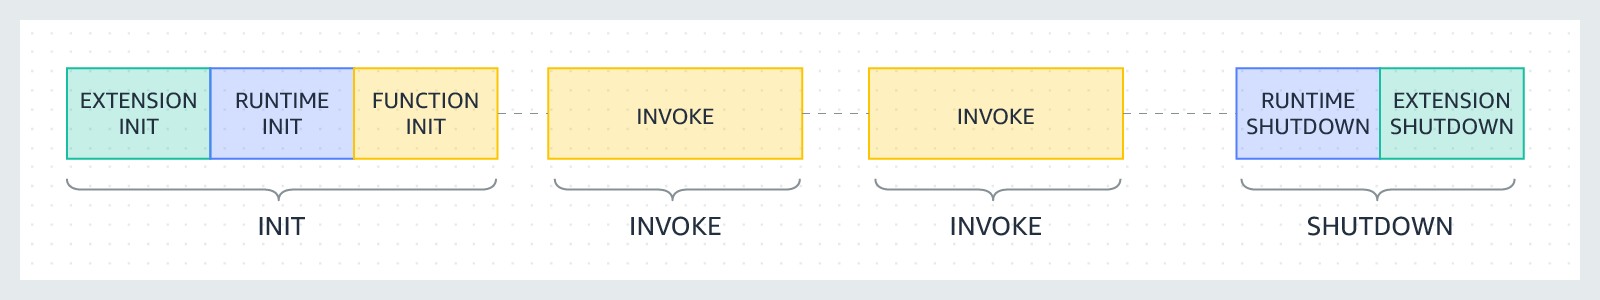
\includegraphics[width=\textwidth]{diagrams/lambda.png}
  \caption{Lambda execution environment lifecycle.}
  \label{fig:pipeline}
\end{figure}

\subsection{Serverless principles}

Serverless is a misnomer, since servers are still in the picture
this computing model must not be confused with other paradigms
that do not require an actual server such as peer-to-peer (P2P).
Instead, it is more accurate to interpret it as "less-server",
therefore emphasizing the shift in architectural responsibility from developers actively
managing server infrastructure to entrusting platform providers to manage the underlying server complexities.


\subsection{Platform providers}

Lorem ipsum dolor sit amet, qui minim labore adipisicing minim sint cillum sint consectetur cupidatat.

\section{Server-side JavaScript}

Lorem ipsum dolor sit amet, qui minim labore adipisicing minim sint cillum sint consectetur cupidatat.

\subsection{TypeScript}

Lorem ipsum dolor sit amet, qui minim labore adipisicing minim
